% Auditing Data Leakage and Reporting Gaps in EEG Connectivity Deep Learning for Depression Detection
% MLESP 2026 (IEEE BIBM workshop). DOUBLE-BLIND: no author names, affiliations or acknowledgements until camera-ready.
%
% BUILD (from 06_Manuscript):  python make_macros.py   then   pdflatex paper; bibtex paper; pdflatex paper; pdflatex paper
% Every number in the text is a macro from macros_counts.tex, generated from the screening log and analysis
% output. Never type a number into this file.
%
% Visible markers that MUST be gone before submission (grep for them):
%   \CITE{...}     a reference still needed - fill only with a paper you have opened (blueprint Sec 12)
%   \PENDING{...}  wording or a number waiting on the advisor or on coding
%   UNVERIFIED     printed in the bibliography until the reference is checked
\documentclass[conference]{../06_Manuscript/template/IEEEtran/IEEEtran}
\usepackage{cite}
\usepackage{amsmath,amssymb}
\usepackage{graphicx}
\usepackage{booktabs}
\usepackage{array}
% CAMERA-READY 2026-11-08: needed for the released-repository URL in Section VII.
\usepackage{url}
\urlstyle{same}

\newcommand{\CITE}[1]{\textbf{[CITE: #1]}}
% REVIEW 2026-09-27 (C8): one switch for advisor-dependent notes. Default FALSE: every note prints and preflight fails.
% Set \decisionsacceptedtrue ONLY after the advisor (or the authors, in writing) accepts every default listed in
% REVISION_NOTES.md, Table "Decisions". It hides the notes; it does not change any sentence of the paper.
% Author inputs always print (preflight flags "AUTHOR:"); they are never hidden by the switch.
\newcommand{\AUTHORINPUT}[1]{\textbf{[AUTHOR: #1]}}
\newif\ifdecisionsaccepted
% 2026-09-27: set TRUE after the advisor signed off on the Decisions table (email of 2026-09-27, 01:47).
\decisionsacceptedtrue
\newcommand{\PENDING}[1]{\ifdecisionsaccepted\unskip\else\textbf{[PENDING: #1]}\fi}
% GENERATED by make_macros.py - do not edit. Re-run after any screening or analysis change.
\newcommand{\NincludedTotal}{18}
\newcommand{\NincludedWos}{14}
\newcommand{\NincludedSupp}{4}
\newcommand{\NwosScreened}{100}
\newcommand{\NwosExclTA}{53}
\newcommand{\NwosSought}{47}
\newcommand{\NwosNotRetrieved}{24}
\newcommand{\NwosAssessed}{23}
\newcommand{\NwosExclFT}{9}
\newcommand{\NexclGeometric}{2}
\newcommand{\NsuppSought}{15}
\newcommand{\NsuppNotRetrieved}{11}
\newcommand{\NsuppAssessed}{4}
\newcommand{\Kappa}{0.91}
\newcommand{\KappaLo}{0.66}
\newcommand{\KappaHi}{1.00}
\newcommand{\PctAgree}{94}
\newcommand{\MedLikely}{98.7}
\newcommand{\MedFree}{88.9}
\newcommand{\CliffDelta}{0.00}
\newcommand{\Nstudies}{18}
\newcommand{\NFree}{3}
\newcommand{\NPossible}{2}
\newcommand{\NLikely}{10}
\newcommand{\NUnclear}{3}
\newcommand{\PctFree}{17}
\newcommand{\PctPossible}{11}
\newcommand{\PctLikely}{56}
\newcommand{\PctUnclear}{17}
\newcommand{\Ntiebreak}{1}
\newcommand{\PctSubject}{33}
\newcommand{\PctUnclearSplit}{17}
\newcommand{\PctUnclearScope}{0}
\newcommand{\PctUnclearThresh}{0}
\newcommand{\PctUnclearNorm}{17}
\newcommand{\PctUnclearSelect}{6}
\newcommand{\PctWholeScope}{0}
\newcommand{\PctWholeThresh}{0}
\newcommand{\PctWholeNorm}{0}
\newcommand{\PctWholeSelect}{17}
\newcommand{\PctWithinScope}{100}
\newcommand{\PctWithinThresh}{33}
\newcommand{\PctWithinNorm}{22}
\newcommand{\PctWithinSelect}{0}
\newcommand{\PctNoneThresh}{67}
\newcommand{\PctNoneNorm}{61}
\newcommand{\PctNoneSelect}{78}
\newcommand{\AgreeSplit}{17}
\newcommand{\AgreeScope}{18}
\newcommand{\AgreeThresh}{17}
\newcommand{\AgreeNorm}{15}
\newcommand{\AgreeSelect}{12}
\newcommand{\NdisagreeInitial}{1}
\newcommand{\Nrecoded}{\textbf{[NOT ESTIMABLE: empty stratum - rewrite this sentence]}}
\newcommand{\AgreeRecoded}{\textbf{[NOT ESTIMABLE: empty stratum - rewrite this sentence]}}
\newcommand{\NsubjMedian}{61}
\newcommand{\NsubjMin}{48}
\newcommand{\NsubjMax}{122}
\newcommand{\NsubjMissing}{0}
\newcommand{\DataMumtaz}{8}
\newcommand{\DataMODMA}{5}
\newcommand{\DataPREDCT}{2}
\newcommand{\DataPrivate}{2}
\newcommand{\DataOther}{1}
\newcommand{\ConnPLV}{2}
\newcommand{\ConnPLI}{2}
\newcommand{\ConnCoh}{1}
\newcommand{\ConnCorr}{4}
\newcommand{\ConnGranger}{2}
\newcommand{\ConnOther}{7}
\newcommand{\ArchCNN}{10}
\newcommand{\ArchGNN}{6}
\newcommand{\ArchTransformer}{0}
\newcommand{\ArchOther}{2}
\newcommand{\YearMin}{2020}
\newcommand{\YearMax}{2025}
\newcommand{\PctEpochLo}{29}
\newcommand{\PctEpochHi}{71}
\newcommand{\PctUnclearAnyLo}{9}
\newcommand{\PctUnclearAnyHi}{45}
\newcommand{\PctFreeLo}{6}
\newcommand{\PctFreeHi}{39}
\newcommand{\PctPossibleLo}{3}
\newcommand{\PctPossibleHi}{33}
\newcommand{\PctLikelyLo}{34}
\newcommand{\PctLikelyHi}{75}
\newcommand{\PctUnclearLo}{6}
\newcommand{\PctUnclearHi}{39}
\newcommand{\NaccStudies}{17}
\newcommand{\NaccFree}{2}
\newcommand{\NaccPossible}{2}
\newcommand{\NaccLikely}{10}
\newcommand{\NaccUnclear}{3}
\newcommand{\MedFreeFmt}{88.9}
\newcommand{\MedPossibleFmt}{94.7}
\newcommand{\MedLikelyFmt}{98.7}
\newcommand{\MedUnclearFmt}{88.6}
\newcommand{\IQRFree}{83.3--94.4}
\newcommand{\IQRPossible}{92.9--96.5}
\newcommand{\IQRLikely}{97.2--99.3}
\newcommand{\IQRUnclear}{87.0--88.8}
\newcommand{\AccFreeValues}{77.8\% and 100.0\%}
\newcommand{\MWU}{10.0}
\newcommand{\MWp}{p = 1.00}
\newcommand{\CliffLo}{$-$1.00}
\newcommand{\CliffHi}{1.00}
\newcommand{\MedDiff}{9.8}
\newcommand{\MedDiffLo}{$-$2.8}
\newcommand{\MedDiffHi}{21.5}
\newcommand{\SESOIverdict}{at least as large as}
\newcommand{\KWH}{3.96}
\newcommand{\KWp}{p = 0.27}
\newcommand{\KWk}{4}
\newcommand{\NLikelySmall}{4}
\newcommand{\NLikelyMedium}{6}
\newcommand{\NLikelyLarge}{0}
\newcommand{\NFreeSmall}{0}
\newcommand{\NFreeMedium}{2}
\newcommand{\NFreeLarge}{1}
\newcommand{\SensOneN}{16}
\newcommand{\SensOneDelta}{0.00}
\newcommand{\SensOneMedDiff}{9.8}
\newcommand{\SensOneNull}{at least as large as}
\newcommand{\SensTwoN}{18}
\newcommand{\SensTwoDelta}{0.33}
\newcommand{\SensTwoMedDiff}{19.0}
\newcommand{\SensTwoNull}{at least as large as}
\newcommand{\SensThreeN}{16}
\newcommand{\SensThreeDelta}{0.00}
\newcommand{\SensThreeMedDiff}{9.2}
\newcommand{\SensThreeNull}{at least as large as}
\newcommand{\SensFourN}{18}
\newcommand{\SensFourDelta}{$-$1.00}
\newcommand{\SensFourMedDiff}{$-$2.7}
\newcommand{\SensFourNull}{smaller than}
\newcommand{\SensOneNfree}{2}
\newcommand{\SensOneNlikely}{8}
\newcommand{\SensTwoNfree}{3}
\newcommand{\SensTwoNlikely}{10}
\newcommand{\SensThreeNfree}{2}
\newcommand{\SensThreeNlikely}{9}
\newcommand{\SensFourNfree}{1}
\newcommand{\SensFourNlikely}{7}
\newcommand{\RqFourRho}{$-$0.52}
\newcommand{\RqFourLo}{$-$0.82}
\newcommand{\RqFourHi}{$-$0.02}
\newcommand{\NgroupStudies}{3}
\newcommand{\PctUnclearAny}{22}
\newcommand{\PctEpoch}{50}
\newcommand{\StrictNfree}{0}
\newcommand{\StrictNfreeBefore}{3}
\newcommand{\StrictNpossible}{5}
\newcommand{\StrictNlikely}{10}
\newcommand{\StrictNchanged}{3}
\newcommand{\StrictNcells}{37}
\newcommand{\KapLone}{0.91}
\newcommand{\KapLoneLo}{0.69}
\newcommand{\KapLoneHi}{1.00}
\newcommand{\AgreeLonePct}{94}
\newcommand{\KapLtwo}{undefined}
\newcommand{\KapLtwoLo}{undefined}
\newcommand{\KapLtwoHi}{undefined}
\newcommand{\AgreeLtwoPct}{100}
\newcommand{\KapLthree}{0.87}
\newcommand{\KapLthreeLo}{0.53}
\newcommand{\KapLthreeHi}{1.00}
\newcommand{\AgreeLthreePct}{94}
\newcommand{\KapLfour}{0.69}
\newcommand{\KapLfourLo}{0.40}
\newcommand{\KapLfourHi}{1.00}
\newcommand{\AgreeLfourPct}{83}
\newcommand{\KapLfive}{0.36}
\newcommand{\KapLfiveLo}{$-$0.05}
\newcommand{\KapLfiveHi}{0.71}
\newcommand{\AgreeLfivePct}{67}
\newcommand{\ClDatasetN}{5}
\newcommand{\ClGroupN}{16}
\newcommand{\ClEpochDsLo}{0}
\newcommand{\ClEpochDsHi}{68}
\newcommand{\ClEpochGrLo}{25}
\newcommand{\ClEpochGrHi}{75}
\newcommand{\ClUnclearDsLo}{0}
\newcommand{\ClUnclearDsHi}{47}
\newcommand{\TopDataset}{Mumtaz}
\newcommand{\TopDatasetN}{8}
\newcommand{\TopDatasetEpoch}{6}
\newcommand{\NepochTotal}{9}
\newcommand{\RqFourPermP}{0.031}
\newcommand{\RqFourOR}{10.0}
\newcommand{\RqFourFisherP}{0.11}
\newcommand{\RqFourNrecent}{6}
\newcommand{\RqFourNincomplete}{6}


\begin{document}
\bstctlcite{IEEEexample:BSTcontrol}

% REVIEW 2026-09-27: title changed at the authors' request (no colon, no "Before the Split").
\title{Auditing Data Leakage and Reporting Gaps in EEG Connectivity Deep Learning for Depression Detection}
% CAMERA-READY 2026-11-07: double-blind review is over, so the author block is restored. Order and
% affiliations are exactly as recorded in PORTAL_title_abstract_plaintext.txt and in the portal record for
% paper S02212. Aledhari is the contact/corresponding author.
\author{
\IEEEauthorblockN{Kunal Chevuri}
\IEEEauthorblockA{\textit{Prosper High School}\\
Prosper, TX, USA\\
kunalchevuri510@gmail.com}
\and
\IEEEauthorblockN{Leah Ileto}
\IEEEauthorblockA{\textit{St.\ Lucy's Priory High School}\\
Glendora, CA, USA\\
leahileto07@gmail.com}
\and
\IEEEauthorblockN{Mohammed Aledhari}
\IEEEauthorblockA{\textit{University of North Texas}\\
Denton, TX, USA\\
Mohammed.Aledhari@unt.edu}
}
\maketitle

\begin{abstract}
% REVIEW 2026-09-27 (C1): rewritten so every claim matches Section V. The earlier draft led with a median comparison
% resting on two leakage-free studies and did not report the main finding (no whole-dataset L2-L4 step reported).
Deep learning applied to electroencephalographic (EEG) functional connectivity is a prominent approach to detecting major depressive disorder (MDD), with reported accuracies often above 90\%. Recent reviews have examined how these studies split data into training and test sets, but not the connectivity pipeline that produces the model input: connectivity estimation, thresholding, normalization, and channel or band selection performed before partitioning can transfer test information into training, and epoch-level partitioning can place segments from one subject on both sides of the split. We define five such leakage surfaces and a four-level risk rating based on reported methods alone, and apply the rating to \NincludedTotal{} studies from a citation-ranked corpus rather than a systematic search, so the figures below describe this corpus and are not prevalence estimates for the literature. The clearest finding is partitioning: \PctEpoch\% of the audited studies partitioned at the epoch rather than the subject level, the surface on which two independent raters agreed most closely ($\kappa = \KapLone$). A further \PctUnclearAny\% left at least one preprocessing step undescribed. No study reported fitting connectivity estimation, thresholds, or normalization on the whole dataset; beyond partitioning, the detectable risk came from selecting channels or bands on all data (\PctWholeSelect\% of studies). Because a step a paper never mentions cannot be distinguished from one never performed, we also report the strictest reading of that convention, under which \StrictNfree{} studies can be verified leakage-free. Only \NaccFree{} studies rated leakage-free reported an eligible accuracy, too few to test whether accuracy differs by rating. We propose an eight-item reporting checklist that lets a reader verify, from the paper alone, that a connectivity pipeline is free of leakage.
\end{abstract}

\begin{IEEEkeywords}
electroencephalography, functional connectivity, deep learning, major depressive disorder, data leakage
\end{IEEEkeywords}

\section{Introduction}
\label{sec:intro}
% Section I - Introduction. SOURCE OF TRUTH (the .md draft is superseded).
% Budget: ~380 for I-A+I-B (option B) or ~300 (option A); see word_budget_MLESP.md, advisor Q2. Cut here and in Section II first if long.

\subsection{Clinical motivation}
% REVIEW 2026-11-07 (space pass, blueprint Sec 9: cut from I and II first). No citation or claim dropped.
Major depressive disorder (MDD) is among the leading causes of disability worldwide \cite{ferrari2013}, yet its diagnosis still rests on clinical interviews and self-report scales of limited test-retest reliability \cite{lin2024,regier2013}. An objective physiological marker would help, and electroencephalography (EEG) is an attractive candidate: affordable, non-invasive, portable, and resolved on the millisecond scale \cite{simmatis2023}. Depression is increasingly understood to involve abnormal communication between large-scale brain networks \cite{kaiser2015}, and functional connectivity---the statistical dependence between signals at different sites, estimated with measures such as coherence, the phase-locking value or the phase lag index---captures that communication from scalp EEG. Deep networks learn from connectivity matrices directly, and a substantial literature applies them to separating people with MDD from healthy controls, many reporting accuracies above 90\% \cite{kaur2025}.

\subsection{The verification problem}
Accuracies of this magnitude would be clinically meaningful if they held. Whether they hold depends on something a reader usually cannot check: whether any information from the test data reached the model during training. This is data leakage, and in neuroimaging machine learning it has been shown to inflate reported performance substantially \cite{rosenblatt2024,yagis2021,lee2023}.

Recent reviews of EEG-based depression detection have examined how studies validate their models---holdout and cross-validation schemes, per-subject and leave-one-subject-out partitioning, and whether models were tested on independent datasets \cite{lin2024,lunaguevara2026}. That is the right question about the split. But a connectivity model does not consume raw EEG. It consumes a connectivity matrix, built through a chain of steps that each run before the split: recordings are epoched, connectivity is estimated, matrices are thresholded into graphs, values are normalized, and channels or frequency bands are selected. Each step can carry test information into training if it draws on data beyond the training fold, and most papers do not report the order of these steps, which leaves the question unanswerable from the paper alone. Fig.~\ref{fig:pipeline} contrasts a leakage-free ordering with a leaking one and marks the five points (L1--L5) at which test information can enter.

% REVIEW 2026-09-27 (E1): core-idea figure placed in the Introduction; IEEE floats it to the top of page 2.
\begin{figure*}[t]
\centering
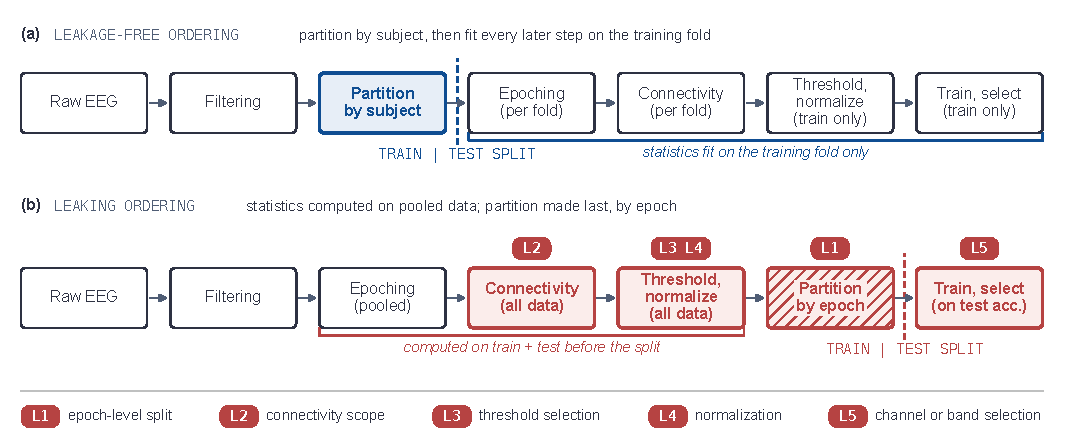
\includegraphics[width=0.74\textwidth]{figures/fig2_pipeline.pdf}
% REVIEW 2026-09-27 (C10)
\caption{The connectivity pipeline with leakage surfaces marked. (a) Leakage-free ordering: data are partitioned by subject before any statistic is computed, and every later step uses the training fold only. (b) Leaking ordering: connectivity (L2) and threshold or normalization statistics (L3, L4) are computed on pooled data, the partition is made by epoch so one subject can fall on both sides (L1), and channels or bands are chosen by test-set accuracy (L5). The dashed line marks the split. Red marks leakage points, hatching the epoch-level partition.}
\label{fig:pipeline}
\end{figure*}


Prior reviews audit how these studies split their data. This work audits what happens to the data before it is split. We searched PubMed, OpenAlex, Semantic Scholar and Google Scholar through September 2026 and found no review that audits connectivity-pipeline construction as a leakage surface in this literature; because that search was not itself conducted as a systematic review, we report it as the limit of our own searching rather than as a claim of priority.
% REVIEW 2026-11-07 (R2 W12): priority claim softened; the search was not systematic, so it cannot support one.

% REVIEW 2026-09-27 (C2): RQ1-RQ4 are used in Sections IV-VII but were never stated. Wording from blueprint RQ list.
We ask four questions. How completely do studies report each leakage surface (RQ1)? Can leakage risk be rated reliably from reported methods by independent raters (RQ2)? Is reported accuracy associated with the rating (RQ3)? And, as a secondary question, does reporting completeness change with publication year (RQ4)?


\subsection{Contributions}
% Worded EXACTLY as blueprint Sec 4. Do not paraphrase.
\begin{enumerate}
  \item A leakage taxonomy for EEG connectivity pipelines. We identify five points at which construction of a connectivity matrix can allow test information into training, and describe the conditions under which each occurs.
  \item A leakage-risk rating scheme. We define a four-level rating applied from reported methods alone, with explicit decision rules, and report inter-rater agreement.
  \item An audit of the literature. We apply the scheme to \NincludedTotal{} studies and report how completely pipelines are described and how reported accuracy varies across risk strata.
  \item A reporting checklist. We propose a short set of items that connectivity-based studies should state so leakage can be ruled out by a reader.
\end{enumerate}

\section{Related Work}
\label{sec:related}
% Section II - Related work. AI DRAFT (Claude, 2026-09-24): Kunal and advisor to edit.
% Budget: ~380 total (option B) or ~300 (option A); see word_budget_MLESP.md, advisor Q2. Per blueprint Sec 9, cut here and in Section I first if long.
% REVIEW 2026-09-27 (C3): wen2020 and young2025 added as design precedents; Yagis random-label clause cut to offset.
% II-A describes corpus studies from their full texts (read during screening). II-B: kaur2025 and zhang2025 are
% described from their ABSTRACTS only (Europe PMC, checked 2026-09-25; full texts are Elsevier, not opened).
% II-C was checked by Claude against the Europe PMC open-access full texts of lee2023 (PMC10547830),
% rosenblatt2024 (PMC10901797) and yagis2021 (PMC8604922) on 2026-09-24. Blueprint Sec 12 still requires Kunal
% to open each original himself; their bibliography entries stay UNVERIFIED until he does.
% 2026-09-25: II-C corrected after KC's own reference check (every correction re-verified by Claude against the
% same full texts): Rosenblatt's leaky covariate regression DEFLATED performance; Yagis's 66->97%
% is the VGG16/OASIS-200 case; Lee's ranges are per model.

\subsection{Deep learning on EEG connectivity for MDD}
In this literature a connectivity measure turns each EEG segment into a channel-by-channel matrix, and a deep network classifies the matrices. Most measures are undirected phase or amplitude couplings (PLV, PLI, coherence, correlation and mutual information) \cite{li2020,dang2020,zhang2023,yu2022,liu2024}; a smaller group uses directed measures from multivariate autoregressive models \cite{saeedi2021,khan2021}. Some stack one matrix per frequency band into a multilayer network \cite{dang2020,sun2022}. Convolutional networks treat the matrix as an image, sometimes with a recurrent branch \cite{saeedi2021,zhang2023,li2024}; graph neural networks treat channels as nodes and connectivity as edge weights \cite{sun2022,sun2024,liu2024}, and recent work learns the graph during training \cite{luo2023,xia2023} or moves it to cortical source space \cite{guo2025}. A few public datasets with tens of participants per group recur (Table~\ref{tab:corpus}). Reported accuracies commonly exceed 95\%, yet these studies seldom state when the pipeline's statistics were computed relative to the train/test split.

\subsection{Existing reviews of validation practice}
% REVIEW 2026-11-07 (C10 space pass, blueprint Sec 9: cut from II before III or V): condensed to free
% room for the reviewer-requested analyses in Sections IV, V and VI. No citation or claim dropped.
Recent reviews compare validation schemes in EEG depression studies; one found none that validated across datasets \cite{lin2024}, another found near-perfect accuracy most often where samples were small and validation subject-dependent \cite{lunaguevara2026}, and a third found that the lack of standardized evaluation protocols limits comparison \cite{kaur2025}. A meta-analysis of 176 machine-learning studies of MDD found reported accuracy negatively correlated with sample size \cite{zhang2025}---the confound this audit addresses through sample-size stratification.

The distinction we draw is one of scope. These reviews ask how a study separated training from test data, and whether its validation was subject-dependent or subject-independent, and one of them also discusses feature selection \cite{lunaguevara2026}. None that we found asks whether the steps that build the connectivity matrix itself---estimation, thresholding and normalization---were fit before that separation. A study can use leave-one-subject-out validation and still leak through a threshold chosen on the pooled data; a review that records only the validation scheme would score it as sound.
% REVIEW 2026-11-07: the \PENDING on this sentence is resolved conservatively. Rather than assert that no
% review covers L5, the claim is narrowed to L2-L4 and lunaguevara2026 is credited for feature selection, so
% the sentence holds whether or not that review's full text covers L5. Nothing here needed new verification.

\subsection{Data leakage in neuroimaging machine learning}
Leakage is well documented in neuroimaging. Across four resting-state fMRI connectome datasets, selecting features on the full dataset and repeating subjects across the split inflated performance most \cite{rosenblatt2024}. In MRI classification, splitting by slice rather than subject raised a VGG16 model's accuracy on one dataset from 66\% to about 97\% \cite{yagis2021}. In resting-state EEG from patients with post-traumatic stress disorder, splitting cropped trials rather than participants inflated balanced accuracy by about 5--15 percentage points for one convolutional network and 15--20 for EEGNet \cite{lee2023}. Segment-based rather than subject-based holdout strongly overestimated accuracy on unseen subjects, and most translational EEG studies surveyed used it \cite{brookshire2024}; in EEG-based schizophrenia detection, about 65\% of studies split by epoch or selected features before partitioning, inflating accuracy by up to about 30\% \cite{racz2026}. None examined how connectivity features are built. The connectome work is the closest analogue, deriving features from pairwise connectivity; the two forms it found most damaging correspond to L5 and L1 here. Rating leakage from reported methods also has precedents: one survey labeled each Alzheimer's study's leakage status from its text \cite{wen2020}, and a scoping review stratified 44 such studies into three risk tiers, finding reported accuracy highest where risk was highest \cite{young2025}. We adapt that approach to the steps that build a connectivity matrix.


\section{Leakage in Connectivity Pipelines}
\label{sec:leakage}
% Section III - Leakage in connectivity pipelines. SOURCE OF TRUTH (the .md draft is superseded).
% The intellectual centre of the paper: per blueprint Sec 9, never cut from here or Section V.
% Budget: ~760 total under option B, 1,045 under option A (word_budget_MLESP.md; advisor Q2). Never cut drafted text here (blueprint Sec 9).

\subsection{Pipeline formalization and connectivity measures}
Let $x_i(t)$ denote the signal recorded at channel $i$, $i = 1,\dots,N$, and let $T$ be the number of samples in an epoch. A connectivity-based classifier does not operate on $x_i(t)$ directly; it operates on a matrix $\mathbf{A} \in \mathbb{R}^{N \times N}$ derived from $x_i(t)$ through a chain of steps---filtering, epoching, connectivity estimation, thresholding, normalization---each of which is fit on some subset of the data. The question this audit asks of each study is which subset that was.

\emph{Magnitude-squared coherence} between channels $i$ and $j$ at frequency $f$ is
\begin{equation}
C_{ij}(f) = \frac{|S_{ij}(f)|^2}{S_{ii}(f)\,S_{jj}(f)},
\end{equation}
where $S_{ij}(f)$ is the cross-spectral density \cite{nunez1997}. $S_{ij}$ is estimated over a window of data; if that window spans samples from both partitions, or is averaged across subjects before the partition is applied, the estimate and every feature derived from it carry information from outside the training fold.

The \emph{phase-locking value} \cite{lachaux1999}, with $\Delta\phi_{ij}(t)$ the instantaneous phase difference between channels $i$ and $j$, is
\begin{equation}
\mathrm{PLV}_{ij} = \frac{1}{T}\left|\sum_{t=1}^{T} e^{\mathrm{j}\,\Delta\phi_{ij}(t)}\right|.
\end{equation}
PLV is bounded in $[0,1]$ and is usually estimated within a single epoch, which limits but does not remove the estimation route: pooling epochs across subjects before computing it still leaks.

The \emph{phase lag index}, $\mathrm{PLI}_{ij} = \left|\left\langle \operatorname{sign}\big(\Delta\phi_{ij}(t)\big)\right\rangle_t\right|$, discounts zero-lag coupling, which volume conduction would otherwise dominate \cite{stam2007}.
% REVIEW 2026-09-27 (C10): display equations inlined for space.

Any of these yields a weighted adjacency matrix $\mathbf{A}$. Matrices are often binarized at a threshold $\tau$ ($A^{\mathrm{bin}}_{ij} = 1$ if $A_{ij} > \tau$, else 0), or reduced to their $k$ strongest edges. If $\tau$ or $k$ is chosen from the distribution of $A_{ij}$ pooled across the full dataset---a common way to fix a target graph density---it is a parameter fit on data that include the test set.

\subsection{A taxonomy of leakage surfaces}
Fig.~\ref{fig:pipeline} shows two orderings of the same pipeline. In the leakage-free ordering (a), the train/test partition is applied immediately after filtering, and every later step is computed separately within each fold. In the leaking ordering (b), the partition is applied last, after epoching, connectivity estimation, and threshold or normalization statistics have been computed on the pooled dataset, so the test set has already shaped the features before the model sees a split. We identify five points at which this can occur.

% REVIEW 2026-09-27 (E1): figure* moved to Section I-B (now Fig. 1).


\textbf{L1 --- Epoch-level partitioning.} A recording contributes many epochs, each treated as a sample. If the train/test or fold assignment is made per epoch rather than per subject, epochs from the same subject appear on both sides. \emph{Leakage-free condition:} every epoch from a subject is assigned to the same side.

\textbf{L2 --- Connectivity estimation scope.} Coherence, PLV, PLI, or another measure is estimated from a window of data. \emph{Leakage-free condition:} each estimate lies entirely within one fold, and no estimate is pooled or averaged across subjects before the partition.

\textbf{L3 --- Threshold selection.} A threshold $\tau$ or edge count $k$ is applied to the matrix. \emph{Leakage-free condition:} $\tau$ or $k$ is fixed a priori or chosen from training-fold statistics only, never from a distribution pooled across the full dataset.

\textbf{L4 --- Feature normalization.} Matrices or derived features are standardized or rescaled. \emph{Leakage-free condition:} normalization statistics are computed on the training fold and applied unchanged to the test fold.

\textbf{L5 --- Channel or band selection.} A subset of electrodes or frequency bands is chosen for the final model. \emph{Leakage-free condition:} the subset is chosen a priori or from training-fold performance only, never by comparing candidate subsets on test-set accuracy.

Section~\ref{sec:methods} turns these conditions into rating rules, and Table~\ref{tab:checklist} (Section~\ref{sec:checklist}) into a checklist a reader can apply.

% REVIEW 2026-11-07 (R2 W5, Q5): scope of the taxonomy stated explicitly, so the checklist is not read as complete.
\emph{Out of scope.} Independent component analysis, artifact subspace reconstruction, re-referencing, bad-channel interpolation and normalization of the matrix itself can also be fit on the full dataset before the split; we excluded them as generic preprocessing, and because the corpus rarely describes them well enough to code. L1--L5 and Table~\ref{tab:checklist} are therefore necessary, not sufficient, for ruling out leakage.

\subsection{Why EEG subject signatures make L1 severe}
L1 deserves separate emphasis because EEG carries stable subject-specific signatures: resting-state recordings, including channel coherence, identify individuals across sessions at least two weeks apart \cite{di2021}. A classifier trained on epochs from a subject who also appears in the test set does not need to learn anything about depression to score well on that subject's test epochs; it can recognize the individual and recall their label. A 2026 preprint reproduced this inflation from shared subjects across five resting-state cohorts, including eyes-closed and eyes-open recordings from the Mumtaz depression dataset \cite{sahuc2026}. The literature under audit typically pairs tens of subjects (median \NsubjMedian{}, Table~\ref{tab:corpus}) with many epochs per subject, which is the regime in which within-subject information dominates a shuffled split. The effect is compounded, not replaced, by L2--L5: even under subject-level partitioning, a connectivity or threshold estimate computed on the whole dataset can still transfer test information into the training features.


\section{Methods}
\label{sec:methods}
% Section IV - Methods. SOURCE OF TRUTH (the .md draft is superseded).
% Budget: ~760 total (option B) or ~620 (option A); see word_budget_MLESP.md, advisor Q2.
% Numbers come from 03_Phase3_Corpus/prisma_counts.json and 05_Phase5_Analysis/analysis.py - never type them by hand.

\subsection{Search and screening}
% REVIEW 2026-11-07 (8-page limit): condensed into one paragraph. No criterion or count dropped.
The starting corpus was a previously assembled set of the 100 most-cited articles returned by a Web of Science search on EEG, connectivity, deep learning and depression. Records were screened on title and abstract, then full text, against six criteria, all of which had to hold: (1) EEG is the primary modality; (2) a functional or effective connectivity measure is computed---coherence, PLV, PLI, correlation, Granger causality, mutual information, or a graph derived from one; (3) a deep learning model is applied to those features; (4) the study classifies depression or predicts its severity; (5) at least one quantitative performance metric is reported; and (6) the work is peer-reviewed, in English, and published in 2015 or later. Criterion 2 required at least one edge weight to depend on the recorded signals, so a graph fixed by electrode positions or an atlas did not qualify however the paper described it. Because fewer than 15 Web of Science studies had qualified, the protocol's supplementary search was run in OpenAlex and PubMed in September 2026; retrieval then stopped once the corpus reached 15, a stopping rule the protocol did not specify, so \NwosNotRetrieved{} screened-in Web of Science reports were never assessed at full text, one because no copy was available to us. Fig.~\ref{fig:prisma} gives the counts and exclusion reasons.

\begin{figure}[t]
\centering
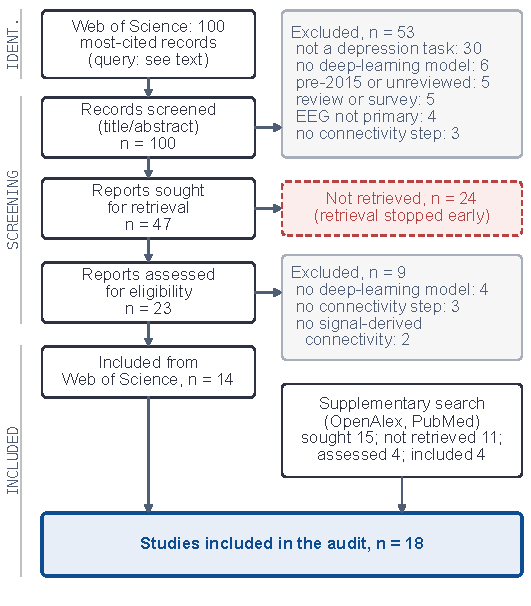
\includegraphics[width=0.80\columnwidth]{figures/fig1_prisma.pdf}
% REVIEW 2026-09-27 (C10): 0.86 width; check legibility
\caption{PRISMA-style screening flow: records at each stage and the reasons for exclusion, generated from the screening log. It is not a systematic review's flow---the starting set was citation-ranked and retrieval incomplete (Section~\ref{sec:discussion}). The supplementary search was run when fewer than 15 studies had qualified, and retrieval stopped at 15 (Section~\ref{sec:methods}). Each of the 100 records is counted once. The dashed box marks reports not retrieved.}
\label{fig:prisma}
\end{figure}

\subsection{Extraction fields}
% REVIEW 2026-11-07 (8-page limit): the three paragraphs below were condensed into two. No field dropped.
The coding sheet's columns were fixed before any study was coded. Descriptive fields recorded the citation; the dataset (MODMA, PRED+CT, the Mumtaz resting-state dataset, a private cohort, or other); total, MDD and control sample sizes; the connectivity measure; the frequency bands; and the architecture family. Pipeline fields recorded whether recordings were epoched and how many epochs each subject contributed; the partitioning unit (subject, epoch, or unclear); and the validation strategy (holdout, $k$-fold, leave-one-subject-out, external, or unclear). Four further fields recorded, for each of L2--L5, whether the step was stated to be fit within the training fold, fit on the whole dataset, not performed, or unclear.

Performance fields recorded reported accuracy and other metrics. Where a study reported more than one accuracy, we took the result for the model the paper proposes under the most subject-independent protocol it reports, coded its leakage fields for that same protocol, and preferred the results tables where these disagreed with the abstract. This rule was fixed after the initial coding pass, which had followed each abstract's headline figure, but before any accuracy was analyzed; one study was left on the protocol both raters coded, with the matching accuracy, so that rating and accuracy always refer to the same protocol. The abstract's headline figure was kept as a second field for a sensitivity analysis. Only binary depression-versus-control accuracies enter the primary comparison; other tasks enter a sensitivity analysis.

% REVIEW 2026-09-27 (E3): rule from the rater guide.
% FIX 2026-09-27 (F1): the last sentence was hidden behind the inline comment above; restored.
% FIX 2026-09-27 (F2): the rater sheets hold one evidence_quote per study, not one per field.
For every study each rater recorded an evidence quote, the passage on which the coding rests. Coding drew only on the published text: authors were not contacted and code repositories were not consulted.

% REVIEW 2026-11-07 (R1 points 1 and 3; R2 W6, Q4): the convention and its direction of bias made explicit,
% with a forward pointer to the bound in Section V-D. The coded fields are unchanged.
One convention needs stating plainly, because it is the weakest point of the scheme. A threshold, rescaling or selection step never mentioned was coded not performed; a step mentioned without saying which data it was fit on was coded unclear. Silence does not establish that a step was not performed, so the convention can only move studies toward the leakage-free end, and our sheets record one value for both readings. We therefore do not rely on it: Section~\ref{sec:results} reports the strictest alternative, treating every such silence as unclear, and states which conclusions survive it.

\subsection{Rating scheme}
Each study received one of four ratings, applied from reported methods alone:
\begin{itemize}
\item \emph{Leakage-free}: subject-level partitioning is stated, and connectivity estimation, thresholding, normalization and channel or band selection are each stated to be confined to the training fold or not performed.
\item \emph{Leakage-possible}: subject-level partitioning is stated, but at least one of L2--L5 is not clearly described as within-fold.
\item \emph{Leakage-likely}: partitioning is at epoch level, or a preprocessing step is explicitly applied to the full dataset before partitioning.
\item \emph{Unclear}: the partitioning unit is not stated.
\end{itemize}
Unclear is a category in its own right rather than missing data, because its prevalence is itself a result for RQ1.

Raters did not assign the rating directly: they coded the partitioning unit and the four surface fields, and a fixed rule implemented in code derived the rating, so both raters' ratings follow the same logic. Where rules overlap, leakage-likely takes precedence: an explicit whole-dataset step makes a study leakage-likely whatever its partitioning unit.

Two conventions were fixed before coding and given to both raters in identical written instructions: a threshold applied to each matrix using only that matrix's own values, and normalization computed within each segment, were coded within-fold, since neither draws on other samples; and batch-normalization layers inside a network were not treated as preprocessing.

\subsection{Rater procedure and analysis plan}
Two raters coded every included study independently, without discussion, from identical written instructions. Percentage agreement and unweighted Cohen's $\kappa$ on the four-level rating were computed before any disagreement was discussed. Disagreements were then resolved with a senior researcher as tiebreaker, and both pre- and post-resolution ratings are reported. A $\kappa$ below 0.4 was pre-specified as indicating that the scheme is too subjective to use as defined.

The analysis was specified, and its code written, before accuracies were examined. RQ1, RQ2 and RQ4 are descriptive and no confirmatory test is performed for them. For RQ1 we report the proportion of studies in each reporting category, overall and per surface, with Wilson 95\% confidence intervals. The 95\% interval for $\kappa$ comes from 10{,}000 bootstrap resamples of studies.

% REVIEW 2026-11-07: the four reviewer-requested analyses are declared here as post hoc, so no reader can
% mistake them for part of the pre-specified plan. Code: 05_Phase5_Analysis/reviewer_response.py.
Four analyses were added after review, once ratings and accuracies were known: the strict re-reading above, per-surface agreement, a bootstrap resampling datasets rather than studies, and an exact test for the year trend. They are post hoc, labeled as such wherever they appear, and changed no coded field, rating or pre-specified result.

RQ3 is the only confirmatory analysis. We report median accuracy and interquartile range per rating stratum and compare the leakage-likely and leakage-free strata with a two-sided Mann--Whitney $U$ test, and all strata with a Kruskal--Wallis test, each accompanied by Cliff's $\delta$ with a 10{,}000-resample bootstrap interval. The smallest effect of interest was fixed in advance at 3 percentage points of median accuracy; a smaller difference is reported as a null, and no subgroup was searched for an effect. Because small datasets may both favor weaker partitioning and yield higher accuracy, accuracy by rating is also reported by sample-size tercile. All resampling used a fixed seed, so every reported value can be regenerated from the coding sheet.


\section{Results}
\label{sec:results}
% Section V - Results. AI DRAFT (Claude, 2026-09-25): Kunal and advisor to edit. Every number is a macro from
% macros_counts.tex (generated by run_pipeline.py), so nothing here is typed by hand.
% Per blueprint Sec 7.5: report in aggregate; never name a study as an example of leakage.
% RESULTS OF 2026-09-25 ARE PROVISIONAL: S11 tiebreak (placeholder = rater A's code), Q20 (binary-only primary),
% Q22 (corpus closed at 18) and S05 (option B) all await the advisor. The interpretive sentences below were written
% for these numbers; if any ruling changes them, re-read every sentence marked "% RECHECK".

\subsection{Corpus characteristics}
The audit included \NincludedTotal{} studies: \NincludedWos{} from the Web of Science set and \NincludedSupp{} from the supplementary search (Fig.~\ref{fig:prisma}). Table~\ref{tab:corpus} lists each. They were published in \YearMin--\YearMax. The Mumtaz resting-state dataset was used by \DataMumtaz{} studies, MODMA by \DataMODMA, PRED+CT by \DataPREDCT{} and a private cohort by \DataPrivate; \DataOther{} used another dataset. The median sample was \NsubjMedian{} subjects (range \NsubjMin--\NsubjMax). Convolutional or recurrent networks were used in \ArchCNN{} studies and graph neural networks in \ArchGNN; Table~\ref{tab:corpus} gives each study's connectivity measure.
% REVIEW 2026-09-27 (C10): measure counts cut for space; they are in Table I.
Because several studies analyzed the same public dataset and \NgroupStudies{} came from one research group, the studies are not fully independent (Section~\ref{sec:discussion}).
% REVIEW 2026-11-07 (R2 W8, Q6): clustering by dataset and research group. POST HOC.
They fall into only \ClDatasetN{} dataset clusters, \TopDataset{} supplying \TopDatasetN{} studies and \TopDatasetEpoch{} of the \NepochTotal{} epoch-level ones, so resampling datasets rather than studies widens the interval on the epoch-level proportion below to \ClEpochDsLo--\ClEpochDsHi\% (post hoc). These proportions describe the corpus, not the literature.

\subsection{Reporting completeness by leakage surface (RQ1)}
In \PctUnclearAny\% of studies the methods did not report enough to determine whether every preprocessing step (L2--L5) was confined to the training fold (95\% CI \PctUnclearAnyLo--\PctUnclearAnyHi\%), and \PctEpoch\% partitioned at the epoch level (\PctEpochLo--\PctEpochHi\%). Fig.~\ref{fig:rq1} gives the distribution for each surface.

% REVIEW 2026-09-27 (C10): the per-surface sentences now repeat Fig. 3, which prints every count and percentage; condensed.
Connectivity was estimated from each segment or subject on its own in every study (L2). Thresholds (L3) and normalization (L4) were either not used or fit per matrix or on training data, except that normalization was not described in \PctUnclearNorm\%. Channel or band selection (L5) drew on all the data in \PctWholeSelect\% and was unclear in \PctUnclearSelect\%.
% RECHECK
The steps specific to connectivity (L2--L4) were never reported as fit on the whole dataset; leakage risk arose instead at partitioning and at selection, and the partitioning unit and the normalization step were the ones most often left undescribed.
% RECHECK
% REVIEW 2026-09-27 (C4): RQ4 moved here from Section VII so no result appears first in the Discussion.
% FIX 2026-09-27 (F4): \RqFourRho holds "$-$0.52"; inside $...$ it printed a text hyphen ("=-0.52"). Now outside math.
% REVIEW 2026-11-07 (R2 W9): exact test added and the interpretation demoted to a hypothesis. POST HOC.
In the secondary analysis (RQ4), reporting completeness fell with publication year (Spearman $\rho =$ \RqFourRho{}, 95\% CI \RqFourLo{} to \RqFourHi), but an exact test on the dichotomized measure does not support it (odds ratio \RqFourOR, Fisher's $p = \RqFourFisherP$, post hoc). From \NincludedTotal{} studies, confounded by venue and design, this is a hypothesis for a larger corpus, not a finding.

\begin{figure}[t]
\centering
\IfFileExists{figures/fig3_rq1.pdf}{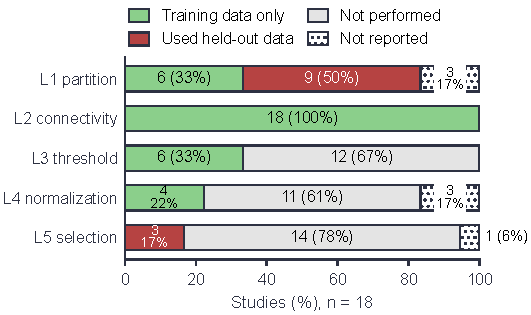
\includegraphics[width=0.95\columnwidth]{figures/fig3_rq1.pdf}}{\fbox{\parbox{0.9\columnwidth}{\centering\PENDING{Fig.~3 is generated by build\_results.py once coding is complete}}}}
\caption{Reporting completeness by leakage surface ($n = \NincludedTotal$). Segments give the number and percentage of studies in which the step was stated to use training data only, stated to use held-out data, not performed, or not reported; for L1, partitioning by subject and by epoch.}
\label{fig:rq1}
\end{figure}

\subsection{Rating distribution and agreement (RQ2)}
Before any discussion, the two raters assigned the same rating to \PctAgree\% of studies, unweighted Cohen's $\kappa = \Kappa$ (95\% CI \KappaLo{} to \KappaHi), above the pre-specified threshold of 0.4. On the individual fields they agreed on \AgreeSplit{} of \Nstudies{} studies for the partitioning unit, \AgreeScope{} for connectivity scope, \AgreeThresh{} for thresholds, \AgreeNorm{} for normalization and \AgreeSelect{} for channel or band selection.
% REVIEW 2026-11-07 (R2 W4, Q3): per-surface kappa added, post hoc. The overall kappa is dominated by the
% common L1 decisions and says nothing about the surfaces that carry the claims.
Because the overall $\kappa$ is dominated by the most common decisions, we also computed it per surface, post hoc: $\kappa = \KapLone$ (95\% CI \KapLoneLo{} to \KapLoneHi) for the partitioning unit, \KapLthree{} for thresholds, \KapLfour{} for normalization, and \KapLfive{} (\KapLfiveLo{} to \KapLfiveHi) for channel or band selection; for connectivity scope every code was identical, so $\kappa$ is undefined. The surface carrying our main result is thus the most reliably coded and selection the least: its $\kappa$ falls below the 0.4 value pre-specified for the overall rating, so every L5 figure here should be read as provisional. Disagreement concentrated there because papers compare bands or channels without saying whether the comparison chose the final model; since the rating follows fixed rules, most field-level disagreements left it unchanged.

% REVIEW 2026-09-27 (C10): duplicate of Methods condensed.
% FIX 2026-09-27 (F1): the tiebreak sentence and the post-resolution rating distribution (RQ2) were hidden behind
% the inline comment above; restored unchanged.
Studies reporting several protocols were handled as described in Section~\ref{sec:methods}. The tiebreaker resolved the remaining disagreement. After resolution, \NFree{} studies (\PctFree\%) were rated leakage-free, \NPossible{} (\PctPossible\%) leakage-possible, \NLikely{} (\PctLikely\%) leakage-likely and \NUnclear{} (\PctUnclear\%) unclear; the 95\% intervals were \PctFreeLo--\PctFreeHi\%, \PctPossibleLo--\PctPossibleHi\%, \PctLikelyLo--\PctLikelyHi\% and \PctUnclearLo--\PctUnclearHi\% respectively.

% REVIEW 2026-11-07 (R1 points 1 and 3; R2 W6, Q4): the bound on the not-reported convention. POST HOC.
\emph{How much the not-reported convention matters (post hoc).} Re-reading every unmentioned threshold, normalization or selection step as unclear rather than not performed---\StrictNcells{} coded cells---moves \StrictNchanged{} studies from leakage-free to leakage-possible, leaving \StrictNfree. The leakage-likely count is unchanged at \StrictNlikely, as is the epoch-level proportion, because both rest on what papers state rather than on what they omit. The convention cannot have inflated the central result, then, but it accounts entirely for the leakage-free count: read strictly, no study here can be verified leakage-free from its methods section.

\subsection{Accuracy by rating (RQ3)}
% RECHECK the whole subsection if the S11 tiebreak, Q20 or S05 changes the numbers. Never change a test or add a subgroup.
The primary comparison used the \NaccStudies{} studies whose recorded accuracy came from a binary depression-versus-control task; one three-class study was excluded from it and enters only the sensitivity analysis.
% REVIEW 2026-11-07 (R2 W14): the 3-versus-2 leakage-free counts reconciled explicitly in the text.
That excluded study is one of the \NFree{} rated leakage-free, which is why \NaccFree{} and not \NFree{} leakage-free studies appear in this comparison. Median reported accuracy was \MedLikely\% (IQR \IQRLikely) among the \NaccLikely{} studies rated leakage-likely and \MedFree\% (the two values were \AccFreeValues) among the \NaccFree{} rated leakage-free, a difference of \MedDiff{} percentage points (bootstrap 95\% CI \MedDiffLo{} to \MedDiffHi; Mann--Whitney $U = \MWU$, \MWp; Cliff's $\delta = \CliffDelta$, 95\% CI \CliffLo{} to \CliffHi). Across all \KWk{} strata, a Kruskal--Wallis test gave $H = \KWH$, \KWp.
The difference in medians exceeds the pre-specified smallest effect of interest of 3 points, but with only \NaccFree{} leakage-free studies, whose median is the midpoint of their two accuracies, it is not distinguishable from zero: the rank-based effect size is null and both intervals include no difference. This comparison is therefore uninformative. It is not evidence that leakage risk is associated with accuracy, nor evidence that it is not.
% RECHECK

Across sample-size terciles (small, medium, large), leakage-likely studies numbered \NLikelySmall/\NLikelyMedium/\NLikelyLarge{} and leakage-free studies \NFreeSmall/\NFreeMedium/\NFreeLarge, too few per cell to compare accuracy within terciles.
% REVIEW 2026-09-27 (C10): condensed % RECHECK
% REVIEW 2026-11-07 (R2 W2; 8-page limit): Fig. 4 (accuracy by rating) REMOVED. It plotted the comparison this
% subsection calls uninformative, and R2 W2 asked for the accuracy comparison to be demoted to a secondary
% role. Dropping it was the one content cut that both frees a float and follows the review. make_fig4_rq3.py
% and the generated PDF are untouched, so the figure can be restored in one line if the advisor prefers.

The pre-specified sensitivity analyses did not change this reading. With one study per research group ($n = \SensOneN$) and without the two weakest inclusions ($n = \SensThreeN$), Cliff's $\delta$ was \SensOneDelta{} and \SensThreeDelta; and including every task ($n = \SensTwoN$) gave $\delta = \SensTwoDelta$; in all three the interval for $\delta$ spanned $-1$ to 1. With each abstract's headline figure, only \SensFourNfree{} study was rated leakage-free, too few for any comparison.
% RECHECK

% Fig. 4 removed 2026-11-07 (see the note above). Restore by reinstating this float and the Fig. 4 reference
% in the sample-size tercile sentence.


% Table I - corpus characteristics (blueprint Sec 10). Generated by build_results.py from the final coding sheet.
\IfFileExists{table_I_body.tex}{% GENERATED by build_table1.py from coding_sheet_FINAL.csv - do not edit by hand.
\begin{table*}[t]
\caption{Corpus characteristics, one row per included study; Study gives the reference number. Ratings describe what each paper reports, not how the study was conducted.}
\label{tab:corpus}
\centering
\scriptsize
\begin{tabular}{lllllrrl}
\toprule
Study & Dataset & $N$ subj. & Connectivity & Architecture & Partition unit & Acc.\ (\%) & \shortstack[l]{Risk rating from\\reported methods} \\
\midrule
\cite{saeedi2021} & Mumtaz & 64 & Granger & CNN-LSTM & epoch & 99.2 & likely \\
\cite{li2020} & private & 48 & coherence & CNN & subject & 80.7 & likely \\
\cite{xia2023} & Mumtaz & 57 & other & CNN & subject & 91.1 & possible \\
\cite{dang2020} & Mumtaz & 64 & PLV & CNN & epoch & 97.3 & likely \\
\cite{zhang2023} & MODMA & 53 & PLI & CNN-LSTM & epoch & 96.3 & likely \\
\cite{luo2023} & PRED+CT & 63 & other & GCN & subject & 77.8 & free \\
\cite{li2024} & Mumtaz & 55 & other & CNN & epoch & 99.9 & likely \\
\cite{sun2024} & MODMA & 53 & other & GCN & epoch & 99.7 & likely \\
\cite{jia2025} & MODMA & 53 & correlation & other & unclear & 89.0 & unclear \\
\cite{zeng2024} & MODMA & 53 & correlation & GCN & epoch & 98.1 & likely \\
\cite{prakash2021} & other & 122 & correlation & LSTM & unclear & 88.6 & unclear \\
\cite{li2023} & private & 67 & PLI & CNN & subject & 79.6$^{a}$ & free \\
\cite{guo2025} & PRED+CT & 120 & other & other & unclear & 85.3 & unclear \\
\cite{yu2022} & Mumtaz & 64 & other & CNN & epoch & 97.2 & likely \\
\cite{liu2024} & MODMA & 53 & correlation & GCN & subject & 98.3 & possible \\
\cite{chen2023} & Mumtaz & 64 & other & GCN & epoch & 99.3 & likely \\
\cite{khan2021} & Mumtaz & 60 & Granger & CNN & subject & 100.0 & free \\
\cite{sun2022} & Mumtaz & 64 & PLV & GCN & epoch & 99.3 & likely \\
\bottomrule
\multicolumn{8}{l}{$^{a}$Not a binary depression-vs-control task; excluded from the primary accuracy comparison (Section V-D).} \\
\end{tabular}
\end{table*}
}{%
\begin{table}[t]\caption{Corpus characteristics}\label{tab:corpus}\centering
\fbox{\parbox{0.9\columnwidth}{\centering\PENDING{Table I is generated by build\_results.py from the final coding sheet}}}
\end{table}}

\section{A Reporting Checklist}
\label{sec:checklist}
% Section VI - A reporting checklist. Table II items are transcribed VERBATIM from blueprint Sec 11
% (advisor content). Do not reword or add items; Sec 14: keep to eight, answerable in about ten minutes.
% Budget: ~220 words of prose plus the table (word_budget_MLESP.md).

% REVIEW 2026-11-07 (8-page limit): the three prose paragraphs condensed into one. No item changed.
Table~\ref{tab:checklist} lists eight items a connectivity-based study should state, one per leakage surface, each answerable in a sentence; together they let a reader decide from the paper alone whether test information could have reached training, a question \PctUnclearAny\% of the audited studies left open for at least one step. For items 5 to 7 what matters is which data a step was fit on, and the epochs per subject (item 2) show how much a subject-identity shortcut could contribute under epoch-level partitioning. The checklist adds no procedure: a study that already partitions by subject and fits every statistic within the training fold satisfies it with a few sentences. Each item should be answered even when the step was not performed, so a reader can tell an omitted step from an undescribed one---a distinction this audit could not draw (Sections~\ref{sec:methods},~\ref{sec:results}).

% REVIEW 2026-11-07 (R2 W11, Q7): relation to existing reporting guidance.
% The TRIPOD+AI and CLAIM entries were REMOVED from references.bib: at the 8-page limit their two reference
% lines were the overflow onto page 9, and blueprint Sec 12 forbids citing a paper no author has opened, which
% there was no time to do. They are named, not cited; only brookshire2024, already verified, carries a citation.
General reporting guidance for prediction models and medical-imaging AI---TRIPOD+AI, CLAIM---already asks for the validation scheme and the handling of predictors, and recommendations for EEG decoding ask for subject-level partitioning \cite{brookshire2024}, but none names the statistics specific to a connectivity matrix. Table~\ref{tab:checklist} replaces none of them; it adds that layer.

\begin{table}[t]
\caption{Reporting checklist for connectivity-based deep learning studies (Gen.\ = generalization)}
\label{tab:checklist}
\centering
\small
\begin{tabular}{@{}r p{0.70\columnwidth} l@{}}
\toprule
\# & A connectivity study should state & Addresses \\
\midrule
1 & Whether data were partitioned by subject or by epoch & L1 \\
2 & The number of subjects and the number of epochs per subject & L1 \\
3 & Whether connectivity was estimated separately within each training fold & L2 \\
4 & The window length and overlap used for connectivity estimation & L2 \\
5 & How any threshold or edge-count parameter was selected, and from which data & L3 \\
6 & Whether feature normalization statistics were computed on training data only & L4 \\
7 & Whether channel or band selection used test-set performance & L5 \\
8 & Whether any external or cross-dataset evaluation was performed & Gen. \\
\bottomrule
\end{tabular}
\end{table}


\section{Discussion and Limitations}
\label{sec:discussion}
% Section VII - Discussion and limitations. AI DRAFT (Claude, 2026-09-25): Kunal and advisor to edit.
% Blueprint Sec 14 REQUIRES: (1) concede directly that this rates reporting, not conduct; (2) state the deviation
% from full systematic-review procedure as a limitation. Sentences marked "% RECHECK" depend on the provisional
% results of 2026-09-25 (S11, Q20, Q22, S05 await the advisor).

% REVIEW 2026-11-07 (8-page limit): condensed. This paragraph restated Section V; it now interprets instead.
The clearest finding concerns partitioning, not the connectivity pipeline itself: \PctEpoch\% of studies split recordings by epoch and \PctUnclearSplit\% did not state the unit, while no study reported fitting connectivity estimation, thresholds or normalization on the whole dataset. What limited verification was omission. The accuracy comparison could not answer RQ3. That absence of evidence should not be read as evidence that leakage leaves accuracy unchanged, which the neuroimaging studies in Section~\ref{sec:related} show it need not, nor should any individual study's accuracy be read as inflated because of its rating.
% RECHECK

% P2 (approved 2026-09-27): the 'connectivity label' paragraph was cut; its fact is in Fig. 2 and criterion 2.

\emph{This audit rates reporting, not conduct.} A study rated unclear or leakage-possible may have run a leakage-free pipeline and not said so; one rated leakage-free may contain an error its text does not reveal. Coding an unmentioned step as not performed overstates how many are leakage-free, which Section~\ref{sec:results} bounds. Our ratings describe what a reader can verify from the paper---the question that matters for how an accuracy should be read---not any author's practice.

The corpus is not the product of a full systematic review. It began from a previously assembled set of the 100 most-cited Web of Science articles on the topic, whose exact query and search date could not be recovered, and citation-ranked sampling favors older and more visible work. Full-text retrieval stopped once the corpus reached the protocol's minimum of 15 studies, a stopping rule the protocol did not specify; as a result \NwosNotRetrieved{} of the \NwosSought{} screened-in Web of Science reports were not assessed (one because no copy was available to us), and \NsuppNotRetrieved{} of the \NsuppSought{} supplementary reports were not retrieved. Which studies entered therefore depended partly on retrieval order and access rather than on the criteria alone. The ratings are also not fully independent, several studies sharing a dataset and \NgroupStudies{} coming from one research group; Section~\ref{sec:results} reports how much the prevalence figures move when datasets or groups, rather than studies, are resampled.
% REVIEW 2026-11-07 (8-page limit): condensed, and the dataset/group sentence folded in, since V-A now carries
% the clustered intervals in full.

% FIX 2026-09-27: author list is Chevuri, Ileto, Aledhari, so both raters (KC, LI) are authors.
Both raters worked from identical written instructions and coded independently, but both are authors of this paper, and the rules, though mechanical, required interpretive conventions for thresholds and normalization fixed in advance (Section~\ref{sec:methods}). No rater outside the author group coded any study and no blinded re-coding was performed; the per-surface agreement in Section~\ref{sec:results} stands in its place, and shows the weakness plainly---partitioning is coded reliably, channel and band selection is not. AI-drafted screening, approved by an author (Acknowledgment), may also have missed studies a second human screener would have caught.
% REVIEW 2026-09-27 (C10): AI sentence removed; the Acknowledgment states it. (E4) screening limitation added.
% FIX 2026-09-27 (F1): the E4 sentence was hidden behind the inline comment; restored unchanged.

% REVIEW 2026-09-27 (E5): availability statement; anonymized for double-blind review
% REVIEW 2026-11-07 (R2 W13, Q8; W10): released now rather than promised, and offered as the per-surface
% exemplars the reviewer asked for. The URL and DOI are author inputs: fill them before upload.
\emph{Availability.} The coding sheet, both raters' codes, the evidence quote for each study, the tiebreak record and all analysis and figure code are at \url{https://github.com/kunalchevuri/eeg-connectivity-leakage-audit}. Those quotes, with the rules in Section~\ref{sec:methods}, let a reader re-rate the corpus.


\section{Conclusion}
\label{sec:conclusion}
% REVIEW 2026-09-27 (C5): median comparison removed to match the abstract.
% Section VIII - Conclusion. AI DRAFT (Claude, 2026-09-24): Kunal and advisor to edit.
% Blueprint Sec 9: two paragraphs, no new claims. Budget ~100 words (word_budget_MLESP.md, advisor Q2).
% Paragraph 1 restates Results with the SAME macros as the abstract and Section V (blueprint Sec 15: identical
% numbers); its wording is kept neutral until the direction of each result is known. Paragraph 2 restates
% the checklist and depends on no result.

We audited \NincludedTotal{} studies applying deep learning to EEG connectivity for depression detection, rating leakage risk from reported methods alone. \PctEpoch\% partitioned by epoch and \PctUnclearAny\% did not report enough to tell whether preprocessing was confined to the training fold; no study reported fitting connectivity estimation, thresholds or normalization on the whole dataset, and with only \NaccFree{} leakage-free studies the accuracy comparison was uninformative. Read strictly, treating an unmentioned step as undescribed rather than absent, \StrictNfree{} studies can be shown leakage-free from their text. A pipeline that cannot be reconstructed from its description cannot be checked for leakage; Table~\ref{tab:checklist} asks for the eight statements that make the check possible.


% Acknowledgment: AI disclosure at submission (ADVISOR RULING 2026-09-24, Q3/Q4: IEEE author guidelines ask for
% AI-generated content to be disclosed in the acknowledgments; a disclosure does not identify the authors, so it is
% compatible with double-blind review). AI DRAFT of the wording: Kunal and advisor to check it against
% 08_Admin/ai_use_log.md so that it is complete and accurate. Contribution statement held until camera-ready.

% RESTORED 2026-09-27 from REVISION_NOTES C6 (lost when the Overleaf copy was set up), tightened to fit 8 pages without
% dropping any disclosure. APPROVED by the advisor 2026-09-27, with the model line as he specified.
% Corrections to the C6 text, each checked against 08_Admin/ai_use_log.md and the session records:
%  - model versions filled from the Claude Code session records (claude-opus-5, claude-opus-5-5, claude-sonnet-5);
%    the pre-submission review used Claude in the claude.ai app (REVISION_NOTES log entry); its model is not logged;
%  - title/abstract screening was approved by an author in bulk, so "which an author approved", not "each approved";
%  - Claude ran the PubMed, OpenAlex and Semantic Scholar searches and drafted the rater instructions (log, Sep 23-24);
%  - Claude drafted or revised text in every section, including VI (table_II_body.tex prose);
%  - Perplexity also drafted reference-check notes (log, 2026-09-26);
%  - "coded" narrowed: AI did extract descriptive metadata, but no AI coded a leakage field or rated a study.
% CAMERA-READY 2026-11-07: the contribution statement was held until camera-ready (double-blind review).
% It names which authors were the two raters, which Reviewer 2 (W3) asked to be explicit, and who arbitrated.
% REVIEW 2026-11-07 (8-page limit): the contribution statement is folded into the Acknowledgment rather than
% carried as its own section. It still names the two raters and the tiebreaker, which is what R2 (W3) asked for.
\section*{Contributions and Acknowledgment}
K.C.\ designed the audit and wrote the protocol, the analysis code and the manuscript. K.C.\ and L.I.\ were the
two raters, each coding every study independently from identical instructions and without discussion. M.A.\
supervised the work and, not being a rater, acted as tiebreaker. All authors approved the final manuscript.

Generative AI was used as follows; the authors reviewed all of it and take responsibility for the content. Claude (Anthropic; Claude Code and claude.ai, with Opus 5, Opus 5.5 and Sonnet 5) drafted the screening decisions, which an author approved; ran the PubMed, OpenAlex and Semantic Scholar searches; drafted the rater instructions; extracted descriptive metadata, which an author checked against each paper (for seven studies the AI instead re-checked the values against the full text); wrote the analysis, table and figure code to a specification fixed before accuracies were examined; drafted or revised text in every section, which the authors edited; and cross-checked cited claims against sources. Perplexity was used to find candidate references, run Google Scholar searches and draft reference-check notes. An author opened and checked every reference. No AI tool coded a leakage field or rated a study.


\bibliographystyle{IEEEtran}
\bibliography{references}

\end{document}
